\cleardoublepage
\chapternonum{攻读博士学位期间取得的科研成果}

\ifthenelse{\equal{\BlindReview}{true}}
{% For blind review
    \section*{以第一作者身份发表论文}
    \begin{enumerate}
        \item 2018 The 3rd International Conference on Information Communication and Signal Processing of IEEE; EI; 2018。
        \item 《生物医学工程学杂志》; EI; 2023。
    \end{enumerate}

    \section*{以第二作者身份(导师一作)发表论文}
    \begin{enumerate}
        \item Pregnancy Hypertension: An International Journal of Women's Cardiovascular Health ; SCI, IF 2.49; 2019。
        \item Hypertension in Pregnancy; SCI, IF 2.00; 2023。
    \end{enumerate}
}
{% For submission
    \section*{期刊论文}
    \begin{enumerate}
        \item \textbf{江锋}, 朱志斌, 张梦鸽, 冯静雯, 徐艺菲, 陈杭. 一种基于新型检测算法的模块化的脉搏波预处理分析系统的设计与实现[J]. 
        生物医学工程学杂志, 2023, 40(3): 529-535.
        \item \textbf{Feng Jiang}, Wanlin Chen, Xinzhong Chen, Ying Feng, Jiajun Miao, Cuicui Jiao, Hang Chen. The Research of 
        Photoplethysmography Morphology: Distincting Preeclampsia with Hierarchical Area Ratio[C]. 
        2018 IEEE 3rd International Conference on Signal and Image Processing, 202-206.
        \item Hang Chen, \textbf{Feng Jiang}, Wanlin Chen, Ying Feng, Shali Chen, Jiajun Miao, Cuicui Jiao, Xinzhong Chen. 
        Distinguishing preeclampsia using the falling scaled slope (FSS) --- a novel photoplethysmographic morphological parameter[J]. 
        Hypertension in Pregnancy, 2023, 42(1): 1-10.(导师一作)
        \item Hang Chen, \textbf{Feng Jiang}, Dan Drzymalski, Wanlin Chen, Ying Feng, Jiajun Miao, Cuicui Jiao, Xinzhong Chen. 
        A novel parameter derived from photoplethysmographic pulse wave to distinguish preeclampsia from non-preeclampsia[J]. 
        Pregnancy Hypertension, 2019, 15: 166-170.(导师一作)
        \item Chen W, \textbf{Jiang F}, Chen X, Feng Y, Miao J, Chen S, Jiao C, Chen H.
        Photoplethysmography‑derived approximate entropy and sample entropy as measures of
        analgesia depth during propofol–remifentanil anesthesia[J]. Journal of Clinical Monitoring
        and Computing, 2021, 35(2): 297-305.
        \item Chen W, \textbf{Jiang F}, Chen X, Feng Y, Miao J, Jiao C, Chen S, Chen H. Photoplethysmography
        response to laryngeal mask airway insertion during propofol-remifentanil anethesia[C].
        Annual International Conference of the Ieee Engineering in Medicine and Biology Society,
        Berlin, 2019: 4664-4668
        \item 陈婉琳, \textbf{江锋}, 陈新忠, 封英, 缪家骏, 焦翠翠, 陈杭. 脉搏波形态学研究及其在子痫前
        期的应用[J]. 天津大学学报(自然科学与工程技术版), 2019, 52(8): 857-861.
        \item Liu Mengxing, \textbf{Jiang Feng}, Jiang He, Ye Shuming, Chen Hang. 
        Low-power, noninvasive measurement system for wearable ballistocardiography in sitting and standing positions[J]. 
        Computers in industry, 2017,91:24-32.
        \item 陈沙利, 张柳依, \textbf{江锋}, 陈婉琳, 缪家骏, 陈杭. 基于多种生理信号的情绪识别研究[J]. 中国医疗器械杂志研究与论著, 2020, 44(4): 283-287.
    \end{enumerate}

    \section*{参与项目}
    \begin{enumerate}
        \item 国家自然科学基金面上项目,81870868,基于光电容积脉搏波特征参数监测全麻中伤害
        性刺激-抗伤害性刺激平衡状态的研究,2019/01-2022/12,62.2 万,已结题,参加。
        \item 横向课题,浙江和也健康科技有限公司,智能床垫电子检测电路和算法开发,嵌入式开发,2015/12-2016/10,已完结。
    \end{enumerate}

    % 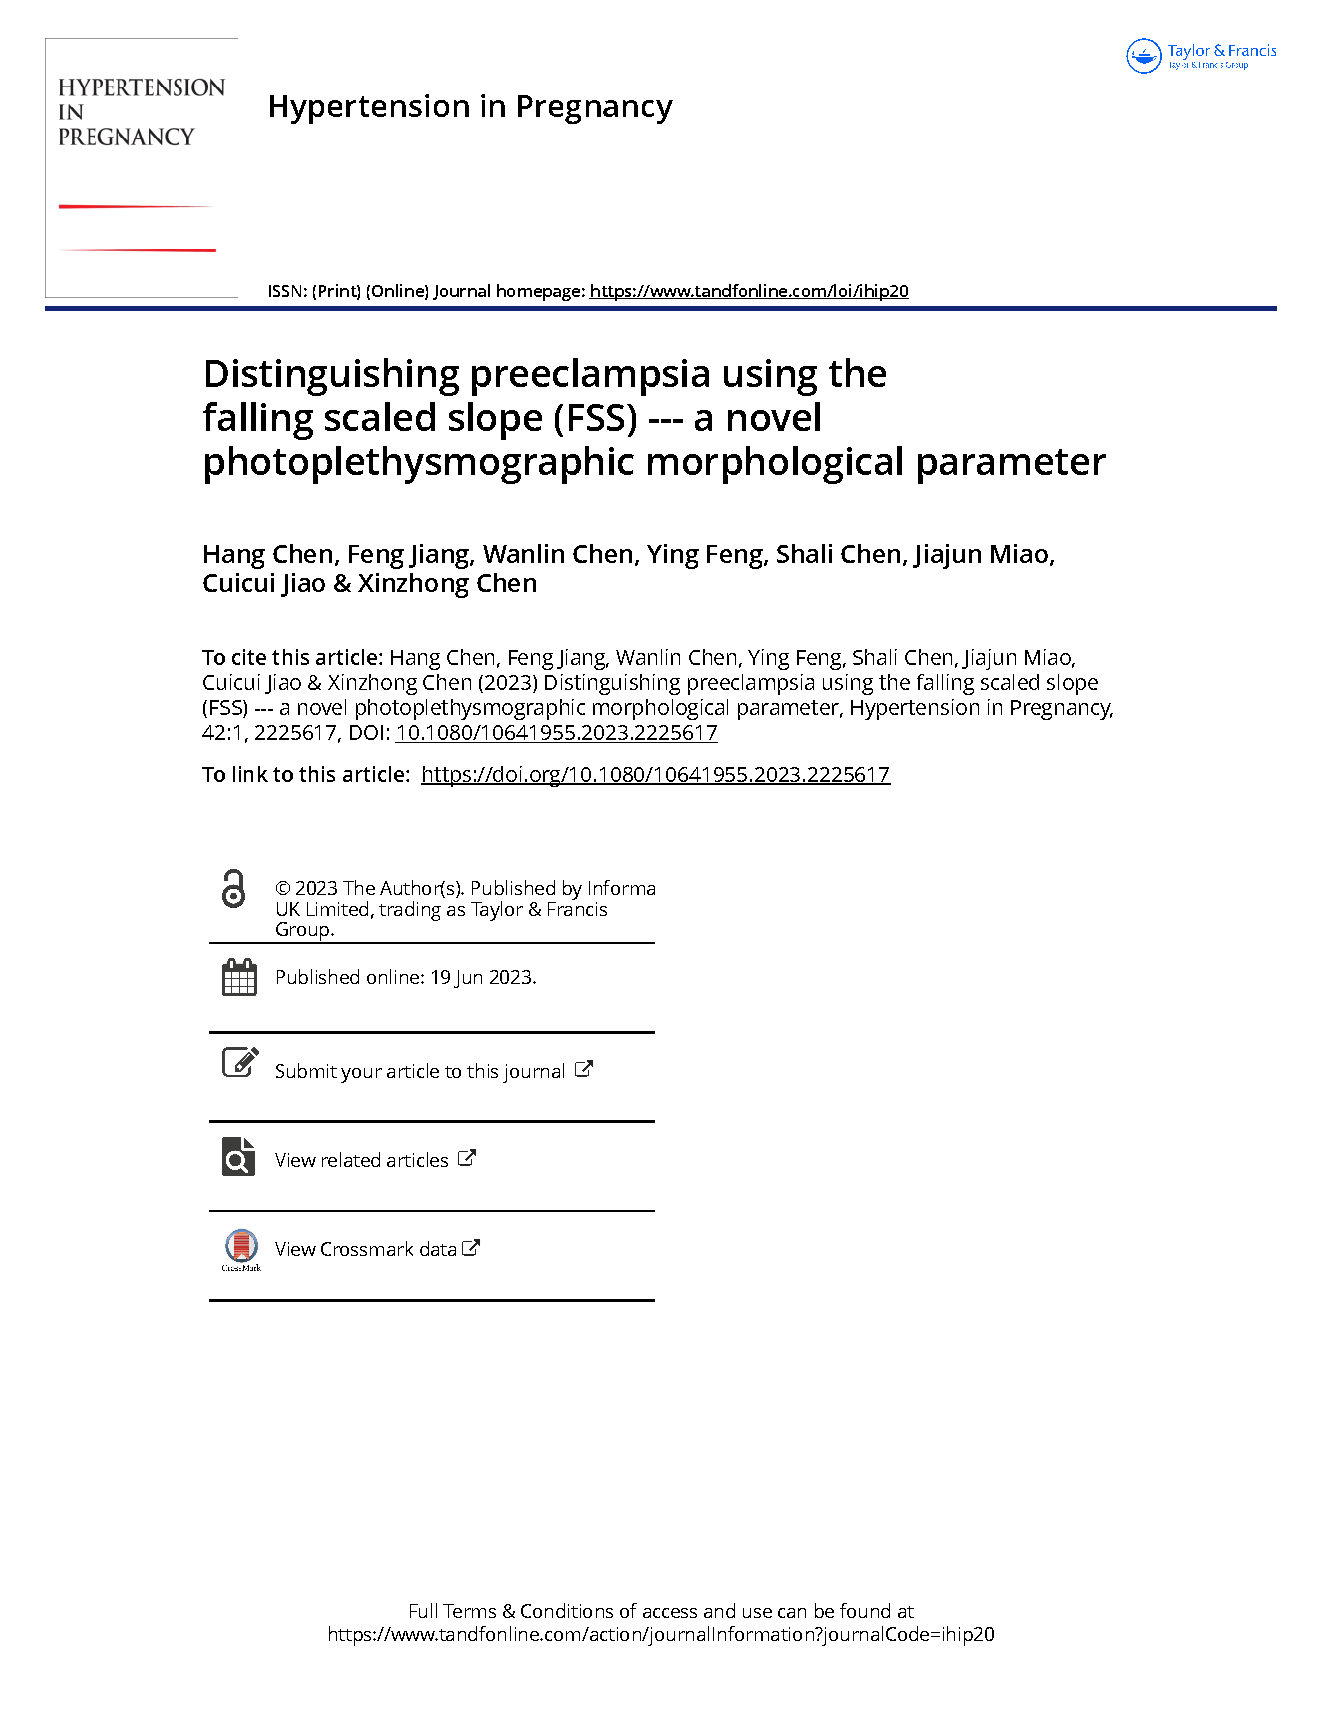
\includepdf[
    %     pages=-,
    %     scale=0.9,
    %     pagecommand={\pagestyle{fancy}},
    %     % frame, % remove this line if you don't want outer fram of pdf
    % ]{papers/sci2.pdf}
    
    % 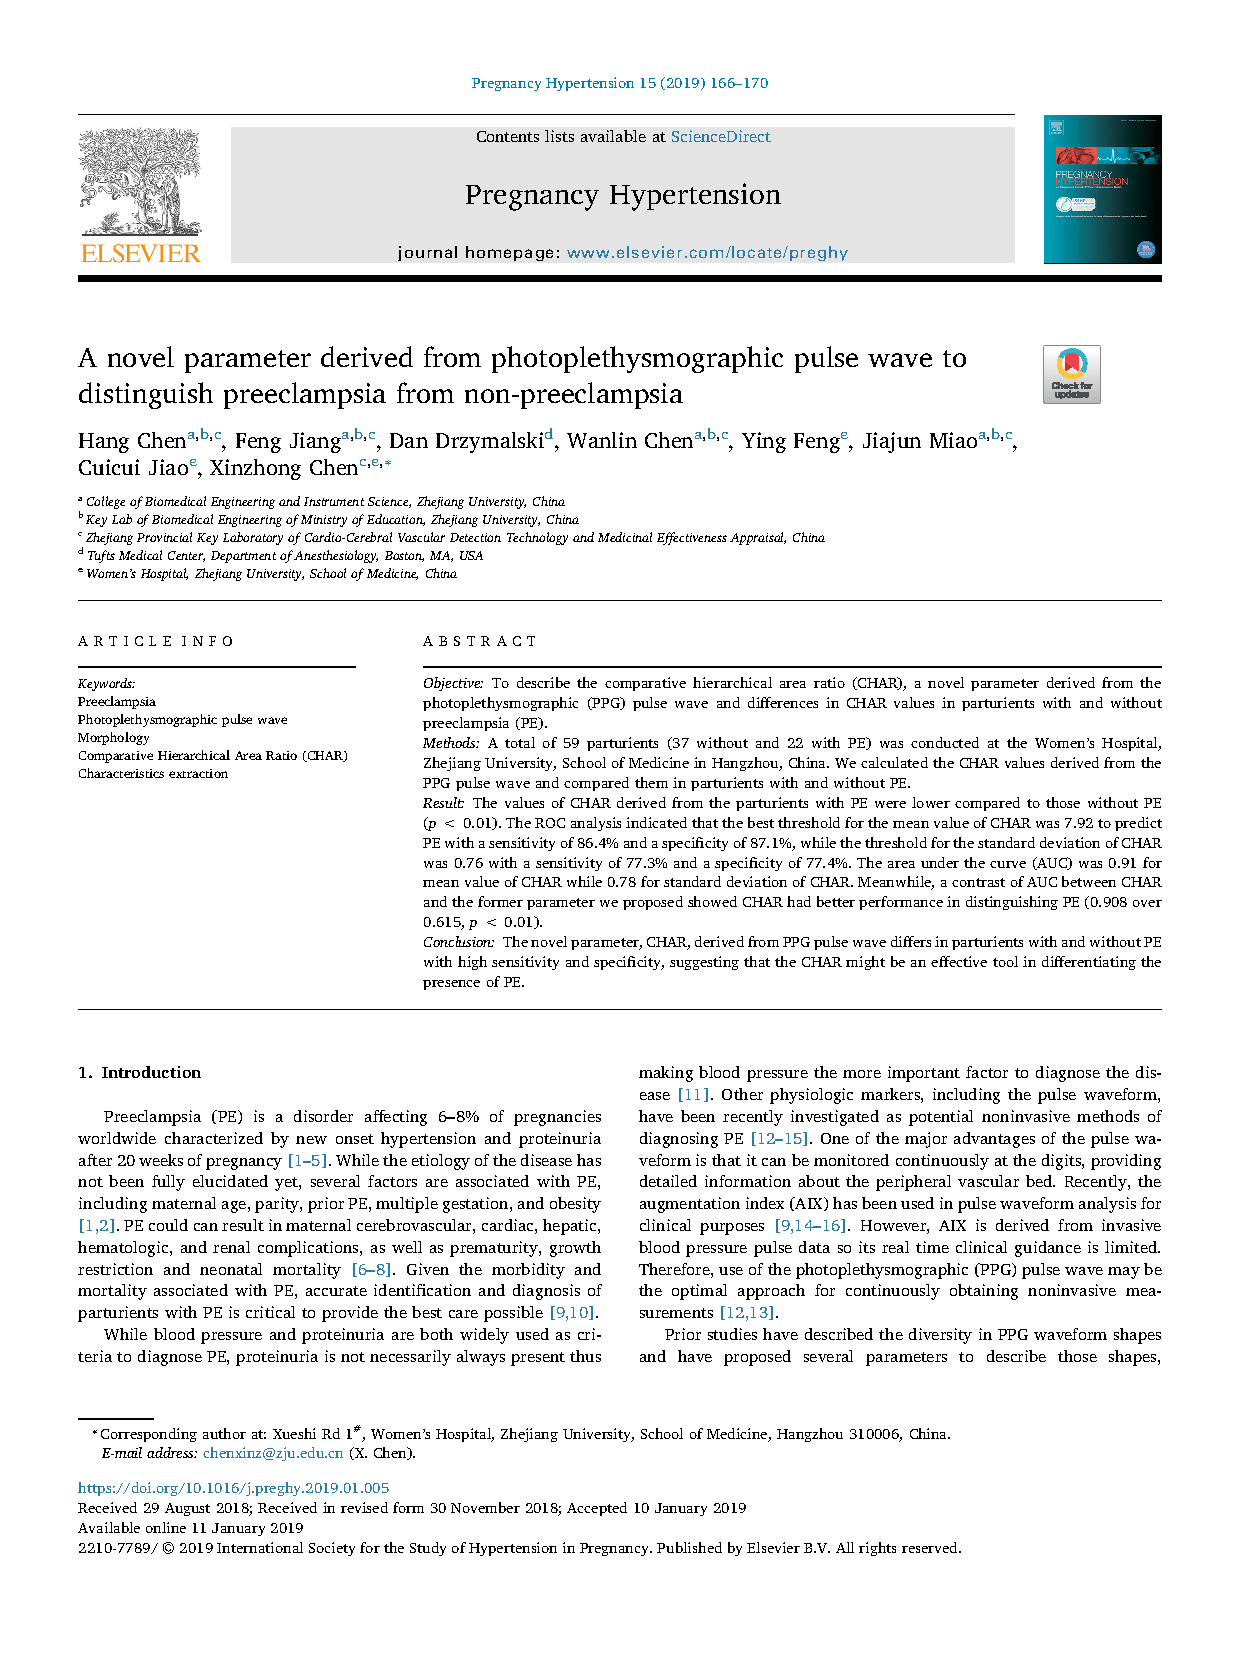
\includepdf[
    %     pages=-,
    %     scale=0.9,
    %     pagecommand={\pagestyle{fancy}},
    %     % frame, % remove this line if you don't want outer fram of pdf
    % ]{papers/sci1.pdf}
    
    % 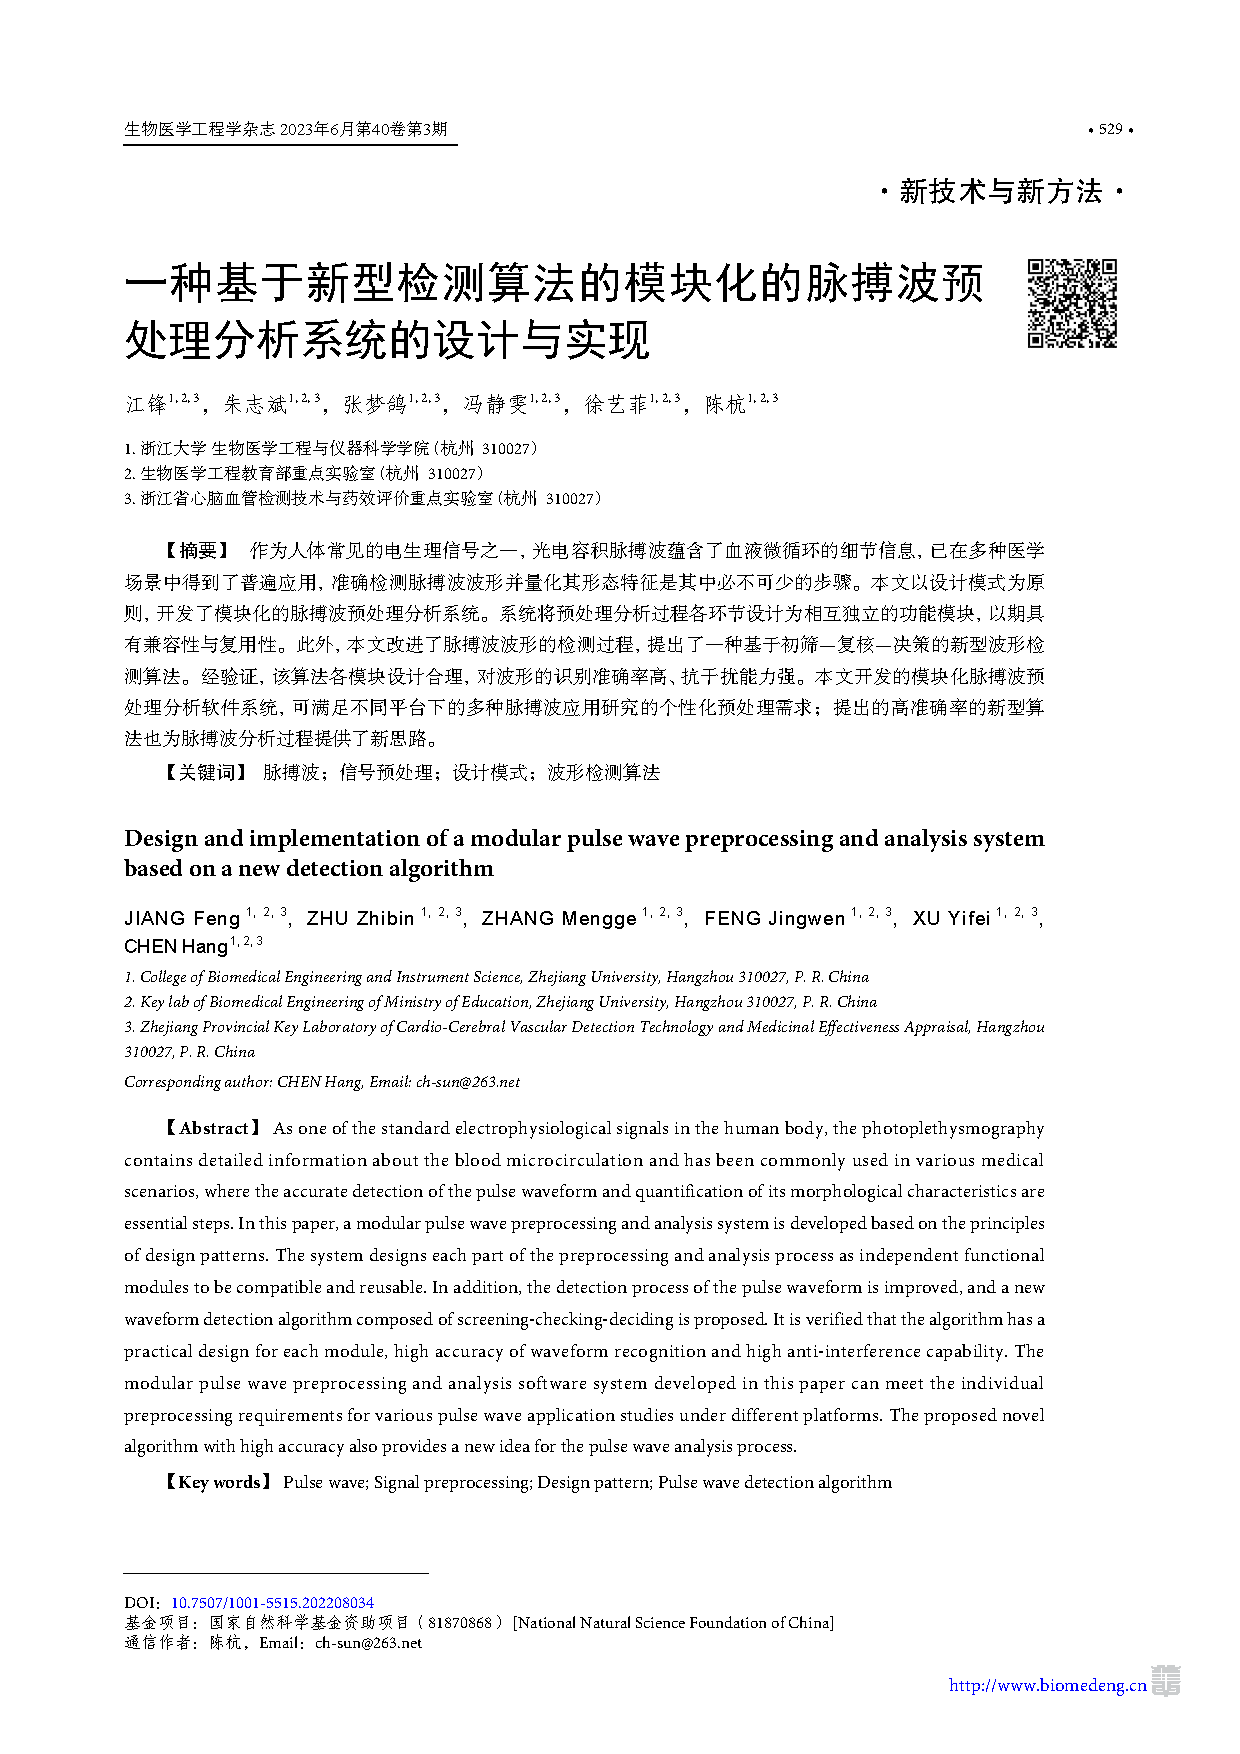
\includepdf[
    %     pages=-,
    %     scale=0.9,
    %     pagecommand={\pagestyle{fancy}},
    %     % frame, % remove this line if you don't want outer fram of pdf
    % ]{papers/ei2.pdf}
    
    % 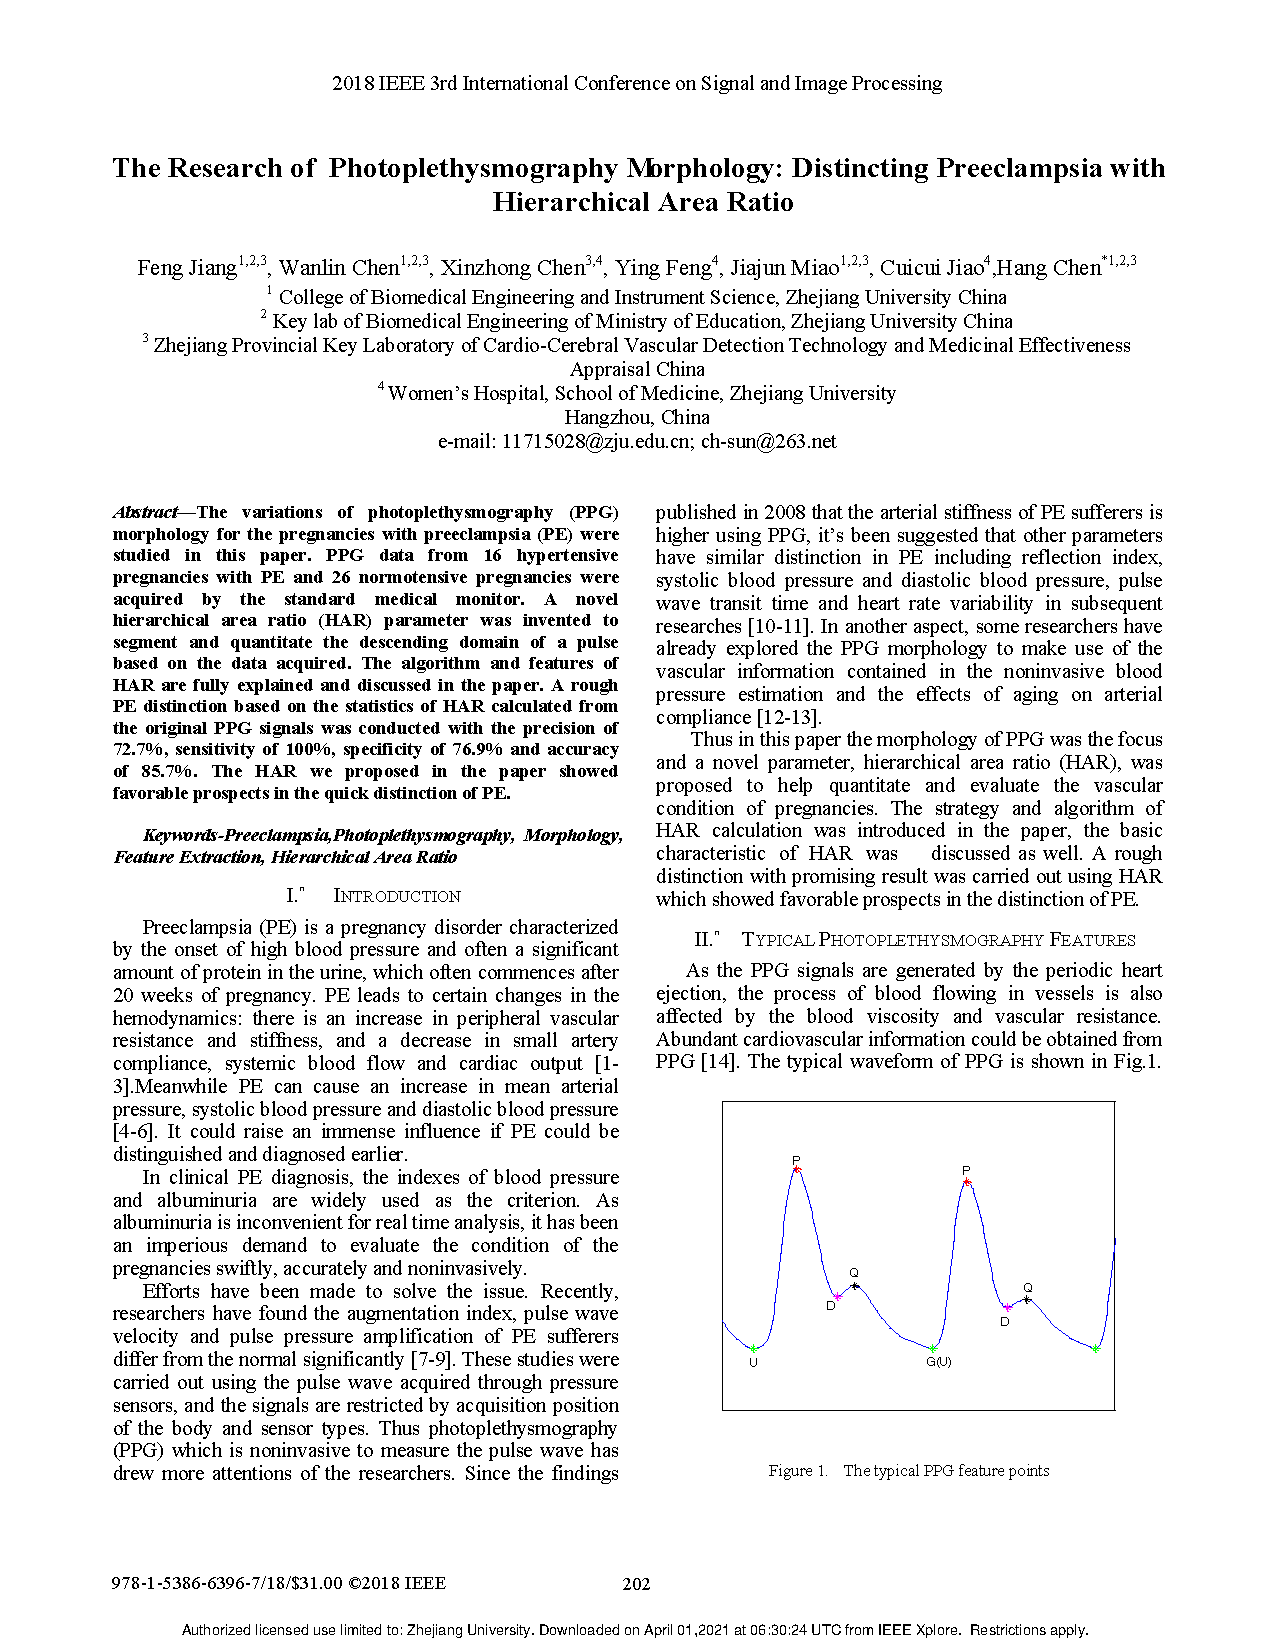
\includepdf[
    %     pages=-,
    %     scale=0.9,
    %     pagecommand={\pagestyle{fancy}},
    %     % frame, % remove this line if you don't want outer fram of pdf
    % ]{papers/ei1.pdf}
}